\documentclass[14pt]{extbook}
\usepackage{multicol, enumerate, enumitem, hyperref, color, soul, setspace, parskip, fancyhdr} %General Packages
\usepackage{amssymb, amsthm, amsmath, latexsym, units, mathtools} %Math Packages
\everymath{\displaystyle} %All math in Display Style
% Packages with additional options
\usepackage[headsep=0.5cm,headheight=12pt, left=1 in,right= 1 in,top= 1 in,bottom= 1 in]{geometry}
\usepackage[usenames,dvipsnames]{xcolor}
\usepackage{dashrule}  % Package to use the command below to create lines between items
\newcommand{\litem}[1]{\item#1\hspace*{-1cm}\rule{\textwidth}{0.4pt}}
\pagestyle{fancy}
\lhead{Progress Quiz 6}
\chead{}
\rhead{Version B}
\lfoot{9689-6866}
\cfoot{}
\rfoot{Spring 2021}
\begin{document}

\begin{enumerate}
\litem{
Write the equation of the line in the graph below in Standard form $Ax+By=C$. Then, choose the intervals that contain $A, B, \text{ and } C$.
\begin{center}
    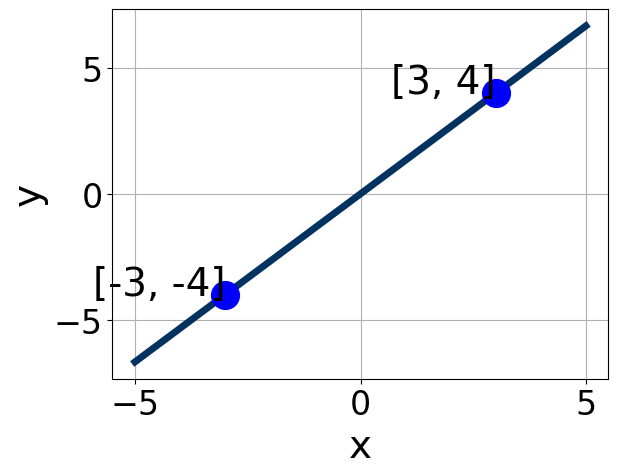
\includegraphics[width=0.5\textwidth]{../Figures/linearGraphToStandardB.png}
\end{center}
\begin{enumerate}[label=\Alph*.]
\item \( A \in [3, 5], \hspace{3mm} B \in [-5.03, -4.97], \text{ and } \hspace{3mm} C \in [-2, 3] \)
\item \( A \in [3, 5], \hspace{3mm} B \in [3.12, 5.64], \text{ and } \hspace{3mm} C \in [-2, 3] \)
\item \( A \in [-1.8, 1.2], \hspace{3mm} B \in [0.01, 1.76], \text{ and } \hspace{3mm} C \in [-2, 3] \)
\item \( A \in [-9, -2], \hspace{3mm} B \in [3.12, 5.64], \text{ and } \hspace{3mm} C \in [-2, 3] \)
\item \( A \in [-1.8, 1.2], \hspace{3mm} B \in [-2.65, -0.66], \text{ and } \hspace{3mm} C \in [-2, 3] \)

\end{enumerate} }
\litem{
Find the equation of the line described below. Write the linear equation as $ y=mx+b $ and choose the intervals that contain $m$ and $b$.\[ \text{Perpendicular to } 9 x + 7 y = 4 \text{ and passing through the point } (-7, 3). \]\begin{enumerate}[label=\Alph*.]
\item \( m \in [0.66, 1.06] \hspace*{3mm} b \in [-9.3, -8.1] \)
\item \( m \in [1.26, 1.34] \hspace*{3mm} b \in [7.3, 9.7] \)
\item \( m \in [0.66, 1.06] \hspace*{3mm} b \in [9.9, 10.9] \)
\item \( m \in [-0.95, -0.68] \hspace*{3mm} b \in [-3.7, -1.3] \)
\item \( m \in [0.66, 1.06] \hspace*{3mm} b \in [7.3, 9.7] \)

\end{enumerate} }
\litem{
First, find the equation of the line containing the two points below. Then, write the equation as $ y=mx+b $ and choose the intervals that contain $m$ and $b$.\[ (3, -6) \text{ and } (-9, 2) \]\begin{enumerate}[label=\Alph*.]
\item \( m \in [-1, 0] \hspace*{3mm} b \in [-4.8, -3.9] \)
\item \( m \in [-1, 0] \hspace*{3mm} b \in [-12.3, -7.9] \)
\item \( m \in [-1, 0] \hspace*{3mm} b \in [0.9, 5.8] \)
\item \( m \in [-1, 0] \hspace*{3mm} b \in [9.9, 12.7] \)
\item \( m \in [-0.2, 1] \hspace*{3mm} b \in [7.2, 10.9] \)

\end{enumerate} }
\litem{
Write the equation of the line in the graph below in Standard form $Ax+By=C$. Then, choose the intervals that contain $A, B, \text{ and } C$.
\begin{center}
    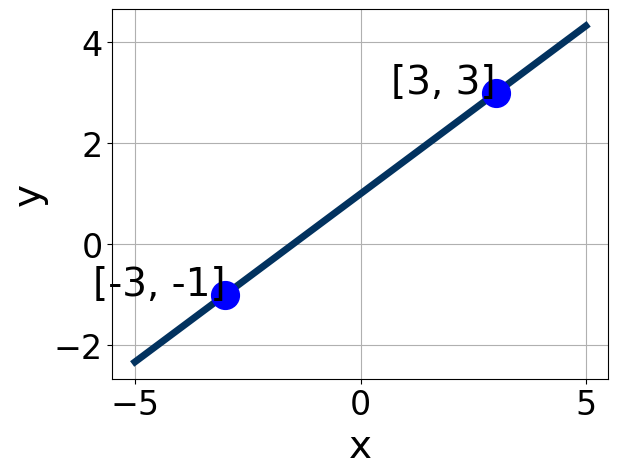
\includegraphics[width=0.5\textwidth]{../Figures/linearGraphToStandardCopyB.png}
\end{center}
\begin{enumerate}[label=\Alph*.]
\item \( A \in [2.93, 4.32], \hspace{3mm} B \in [-2.8, -1.34], \text{ and } \hspace{3mm} C \in [-7, 5] \)
\item \( A \in [-2.44, -0.87], \hspace{3mm} B \in [0.99, 1.1], \text{ and } \hspace{3mm} C \in [-7, 5] \)
\item \( A \in [-3.12, -2.53], \hspace{3mm} B \in [1.46, 2.3], \text{ and } \hspace{3mm} C \in [-7, 5] \)
\item \( A \in [-2.44, -0.87], \hspace{3mm} B \in [-1.65, -0.5], \text{ and } \hspace{3mm} C \in [-7, 5] \)
\item \( A \in [2.93, 4.32], \hspace{3mm} B \in [1.46, 2.3], \text{ and } \hspace{3mm} C \in [-7, 5] \)

\end{enumerate} }
\litem{
Solve the equation below. Then, choose the interval that contains the solution.\[ -13(19x -9) = -11(10x + 3) \]\begin{enumerate}[label=\Alph*.]
\item \( x \in [-0.71, -0.6] \)
\item \( x \in [0.1, 0.26] \)
\item \( x \in [0.81, 1.23] \)
\item \( x \in [0.29, 1.05] \)
\item \( \text{There are no real solutions.} \)

\end{enumerate} }
\litem{
Solve the linear equation below. Then, choose the interval that contains the solution.\[ \frac{5x -5}{6} - \frac{6x -5}{4} = \frac{-9x -9}{8} \]\begin{enumerate}[label=\Alph*.]
\item \( x \in [0.5, 4.9] \)
\item \( x \in [-20.5, -18.9] \)
\item \( x \in [-4.4, -3.2] \)
\item \( x \in [-1.5, 0.3] \)
\item \( \text{There are no real solutions.} \)

\end{enumerate} }
\litem{
First, find the equation of the line containing the two points below. Then, write the equation as $ y=mx+b $ and choose the intervals that contain $m$ and $b$.\[ (-4, 10) \text{ and } (3, -5) \]\begin{enumerate}[label=\Alph*.]
\item \( m \in [-3.14, -1.14] \hspace*{3mm} b \in [10.9, 15.7] \)
\item \( m \in [-3.14, -1.14] \hspace*{3mm} b \in [-2.9, -0.3] \)
\item \( m \in [-3.14, -1.14] \hspace*{3mm} b \in [-10.6, -6] \)
\item \( m \in [0.14, 6.14] \hspace*{3mm} b \in [-13.5, -11.3] \)
\item \( m \in [-3.14, -1.14] \hspace*{3mm} b \in [-1.3, 2.2] \)

\end{enumerate} }
\litem{
Find the equation of the line described below. Write the linear equation as $ y=mx+b $ and choose the intervals that contain $m$ and $b$.\[ \text{Perpendicular to } 3 x - 7 y = 4 \text{ and passing through the point } (-4, -8). \]\begin{enumerate}[label=\Alph*.]
\item \( m \in [-3.6, -2.2] \hspace*{3mm} b \in [-5, -2] \)
\item \( m \in [-1.2, 0.4] \hspace*{3mm} b \in [-20.33, -13.33] \)
\item \( m \in [2.2, 2.5] \hspace*{3mm} b \in [-3.67, 7.33] \)
\item \( m \in [-3.6, -2.2] \hspace*{3mm} b \in [-20.33, -13.33] \)
\item \( m \in [-3.6, -2.2] \hspace*{3mm} b \in [16.33, 22.33] \)

\end{enumerate} }
\litem{
Solve the linear equation below. Then, choose the interval that contains the solution.\[ \frac{4x -5}{8} - \frac{8x + 7}{5} = \frac{-7x + 9}{7} \]\begin{enumerate}[label=\Alph*.]
\item \( x \in [-5.11, -4.11] \)
\item \( x \in [-213, -209] \)
\item \( x \in [1.1, 6.1] \)
\item \( x \in [-36.11, -29.11] \)
\item \( \text{There are no real solutions.} \)

\end{enumerate} }
\litem{
Solve the equation below. Then, choose the interval that contains the solution.\[ -6(-4x + 19) = -13(15x + 2) \]\begin{enumerate}[label=\Alph*.]
\item \( x \in [-0.92, -0.74] \)
\item \( x \in [0.29, 0.43] \)
\item \( x \in [0.58, 0.77] \)
\item \( x \in [-0.8, -0.57] \)
\item \( \text{There are no real solutions.} \)

\end{enumerate} }
\end{enumerate}

\end{document}